\documentclass[preview,border=0pt]{standalone}
\usepackage{tikz}
\usepackage[siunitx,RPvoltages]{circuitikz}
\begin{document}
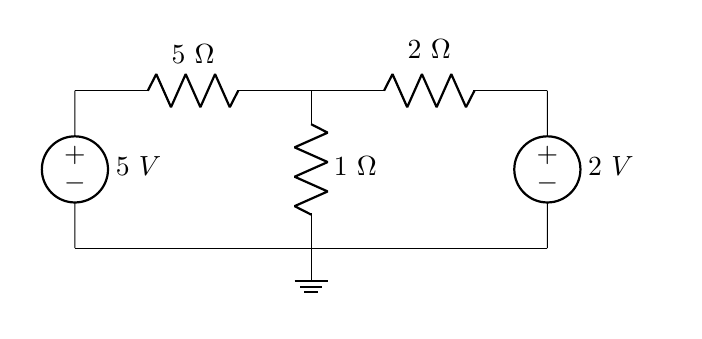
\begin{tikzpicture}
\useasboundingbox (4.4,5.2) rectangle (12.6,8.8);
\draw (5, 8) to[american voltage source, invert, l={$5 \ V$}] (5, 6);
\draw (11, 8) to[american voltage source, invert, l={$2 \ V$}] (11, 6);
\draw (5, 8) to[american resistor, l={$5 \ \Omega$}] (8, 8);
\draw (8, 8) to[american resistor, l={$1 \ \Omega$}] (8, 6);
\draw (8, 8) to[american resistor, l={$2 \ \Omega$}, label distance=0.06cm] (11, 8);
\draw (11, 6) |- (5, 6);
\node[ground] at (8, 6){};
\end{tikzpicture}
\end{document}
